\section*{Аннотация}
В работы мы, измерив диаметр колец Ньютона, определили радиус кривизны линзы. Рассмотрели явление биений желтой и зеленой линии спектра. Определили разность длин волн этих спектральных линий.

\subsection*{Цель работы}
Познакомиться с явлением интерференции в тонких
плёнках (полосы равной толщины) на примере колец Ньютона и с
методикой интерференционных измерений кривизны стеклянной поверхности.
\section*{Теоретические сведения}
\indent Кольца Ньютона представляют собой интерференцию волн, отражённых от границ тонкой 
воздушной прослойки, образованной сферической поверхностью линзы и плоской
стеклянной пластиной. При нормальном падении света интерференционные полосы 
локализованы на сферической поверхности и являются полосами равной толщины.

\begin{wrapfigure}{l}{0.3\linewidth}
    \centering
    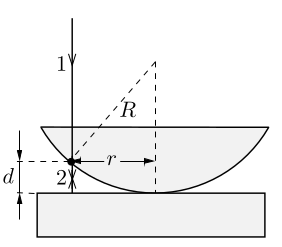
\includegraphics[width=4cm]{images/theory.png}
    \caption{Схема наблюдения колец Ньютона}
\end{wrapfigure}

\indent
Найдем оптическую разность хода интерферирующих лучей. C учетом того, что $R \gg d$:
$$r^2 = R^2 - (R - d)^2 \approx 2Rd \quad \Rightarrow \quad d = \frac{r^2}{2R}$$ 
Тогда выражение для разности хода лучей с учетом потери полуволны при отражении от оптически более плотной среды:
\begin{equation}
    \Delta = 2d + \frac{\lambda}{2} = \frac{r^2}{R} + \frac{\lambda}{2}
\end{equation}
Условие интерференционного минимума:
\begin{equation}
    \Delta = (2m + 1)\frac{\lambda}{2}
\end{equation}
Отсюда получаем радиус темных и светлых колец соответственно:
\begin{equation}
    r_m = \sqrt{m\lambda R} \label{eq:min_radius}
\end{equation}

\begin{equation}
    r_m' = \sqrt{(2m - 1)\lambda R/ 2}\label{eq:max_radius}
\end{equation}

\section*{Экспериментальная установка}
\textbf{Оборудование:} \textit{измерительный микроскоп с опак-иллюминатором; плосковыпуклая линза; пластинка из чёрного стекла;
ртутная лампа ДРШ; щель; линзы; призма прямого зрения; объектная шкала.}

\begin{figure}[h!]
    \centering
    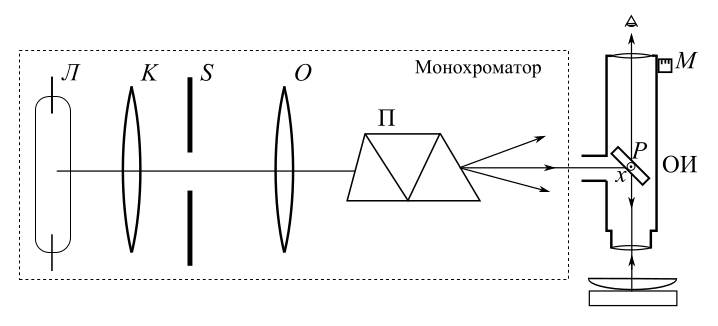
\includegraphics[width=12cm]{images/setup.png}
    \caption{Схема экспериментальной установки}
\end{figure}

Схема экспериментальной установки приведена на рис. 2. Опыт выполняется с помощью измерительного микроскопа.

На столик микроскопа помещается держатель с полированной пластинкой из чёрного стекла. На пластинке лежит исследуемая линза.

Источником света служит ртутная лампа, находящаяся в защитном кожухе. Для получения монохроматического света применяется призменный монохроматор, состоящий из конденсора К, коллиматора (щель S и объектив O) и призмы прямого зрения P. Эти устройства с помощью рейтеров располагаются на оптической скамье.

Свет от монохроматора попадает на расположенный между объективом и окуляром микроскопа опак-иллюминатор (ОИ) — специальное устройство, служащее для освещения объекта при работе в отражённом свете. Внутри опак-иллюминатора находится полупрозрачная стеклянная пластинка P, наклонённая под углом 45° к оптической оси микроскопа. Свет частично отражается от этой пластинки, проходит через объектив микроскопа и попадает на исследуемый объект.

Оптическая схема монохроматора позволяет получить в плоскости входного окна опак-иллюминатора достаточно хорошо разделённые линии спектра ртутной лампы.

Интерференционная картина не зависит от показателя преломления линзы и определяется величиной зазора между линзой и пластинкой (кольца равной толщины).
Cначала микроскоп настраивается на кольца Ньютона в белом свете (свете ртутной лампы), затем при помощи монохроматора выделяется из спектра яркая зелёная линия и проводятся измерения диаметров колец в монохроматическом свете.

\section*{Ход работы}

\subsection*{Калибровка окулярной оси}

Для определения цены деления окулярной шкалы положим сверху на линзу калиброванную объектную шкалу. Плавно поднимая тубус микроскопа, настроимся на стеклянную поверхность шкалы (штрихи, царапины). Перемещая столик, найдем изображение миллиметровой шкалы, совместим его с окулярной шкалой и добъемся наибольшей чёткости.

Объектная шкала размером 1 мм разбита на 100 делений. Одно деление окулярной шкалы равно $a_r = 0.1$ мм. Тогда инструментальная погрешность измерений радиуса будет равна $\sigma_r = 0.005$ мм.

\begin{figure}[h!]
    \centering
    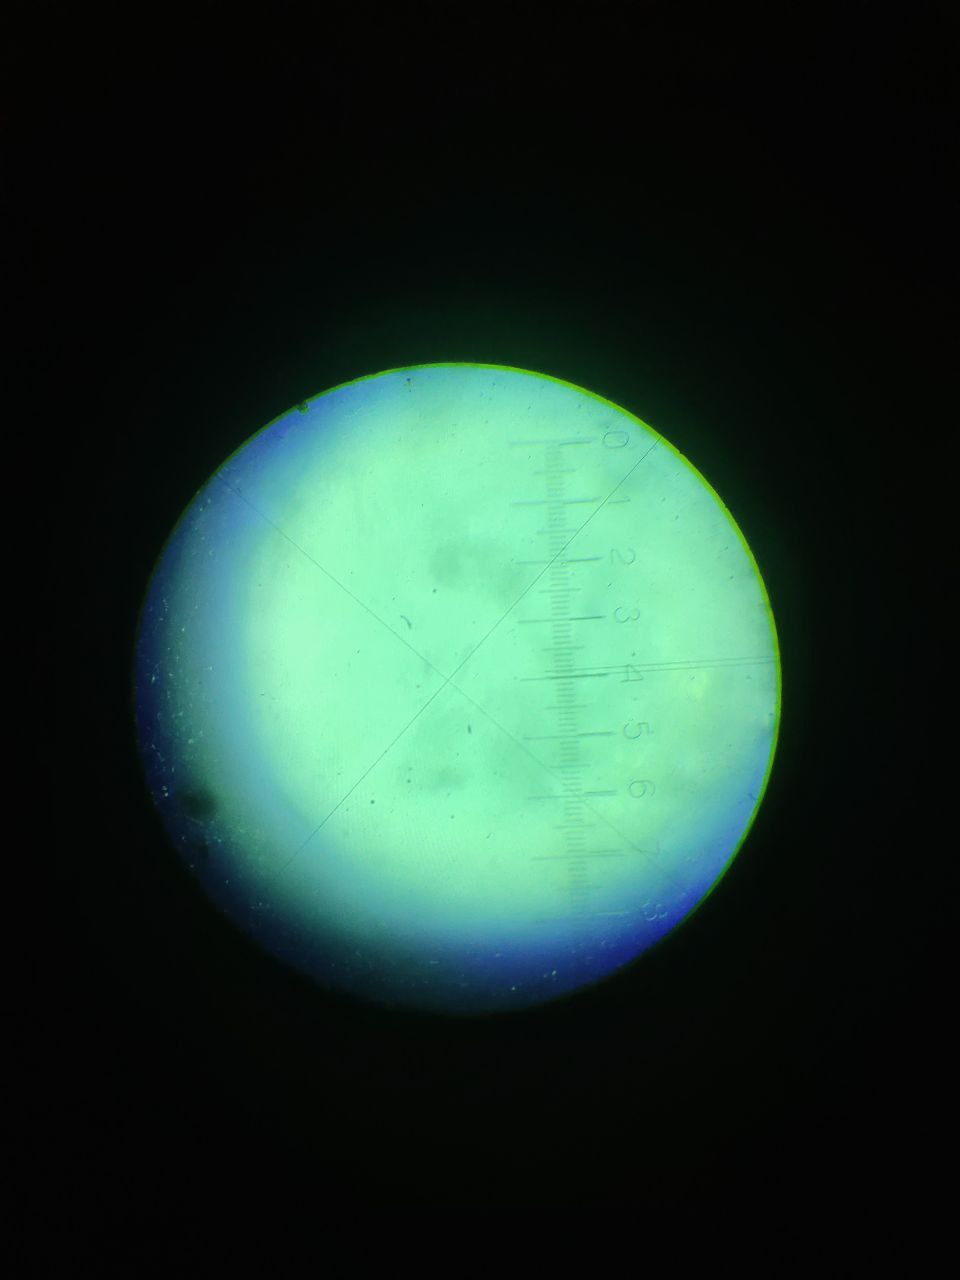
\includegraphics[width=12cm]{images/shkala.jpg}
    \caption{Калибровка окулярной оси}
\end{figure}

\subsection*{Определение радиуса кривизны линзы}
Перемещая перекрестие, последовательно установим его на середины тёмных и светлых колец и запишем соответствующие показания окулярной шкалы и микрометра. После прохождения через центральное пятно продолжим измерения, записывая возрастающие номера колец и координаты их диаметров.

Оценим систематическую погрешность измерения величин на окуляре как $ \sigma_i = 0.02 $ (из-за цены деления).

Оценим диаметр пятна соприкосновения линзы со стеклянной пластинкой.

\begin{table}[h!]
\centering
\begin{tabular}{|c|cc|c|cc|c|}
\hline
$m$ & \multicolumn{2}{c|}{Темные кольца} & $r_m^2$ & \multicolumn{2}{c|}{Светлые кольца} & $(r_m')^2$ \\
\hline
 & $l_1$ & $l_2$ &  & $l_1$ & $l_2$ &  \\
\hline
0 & 4.71 & 3.72 & 0.25 & 4.15 & 4.15 & 0 \\
1 & 5 & 3.24 & 0.77 & 4.78 & 3.43 & 0.46 \\
2 & 5.45 & 2.92 & 1.6 & 5.16 & 3.08 & 1.08 \\
3 & 5.59 & 2.65 & 2.16 & 5.44 & 2.79 & 1.76 \\
4 & 5.83 & 2.42 & 2.91 & 5.7 & 2.54 & 2.5 \\
5 & 6.02 & 2.23 & 3.59 & 5.91 & 2.32 & 3.22 \\
6 & 6.17 & 2.06 & 4.22 & 6.09 & 2.11 & 3.96 \\
7 & 6.47 & 1.89 & 5.24 & 6.25 & 1.97 & 4.58 \\
\hline
\end{tabular}
\caption{Измерение диаметров колец Ньютона}
\label{tab:newton_rings}
\end{table}

Из формул \ref{eq:max_radius} и \ref{eq:min_radius} видно, что квадрат радиуса темных и светлых полос должны линейно зависеть от 
порядка максимума или минимума колец.
\begin{figure}[h!]
    \centering
    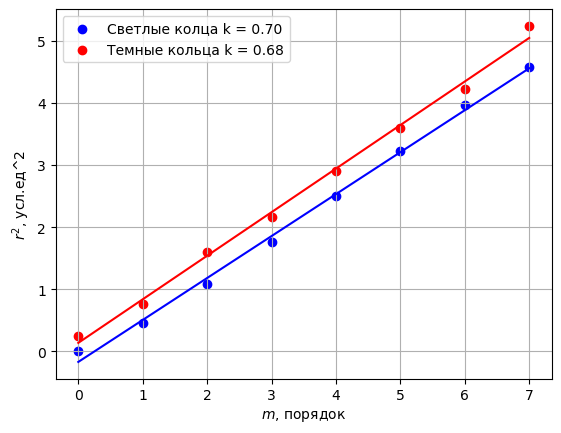
\includegraphics[width=12cm]{images/plot1.png}
    \caption{Зависимость квадратов радиусов колец от их номера}
\end{figure}

$$
R = \frac{r_m^2}{m\lambda} = \frac{0.69 \cdot 0.1^2}{546 \cdot 10^{-6}} = (12.6 \pm 0.2)  \text{мм}
$$


\subsection*{Наблюдение биений}

Осветим входное окно опак-иллюминатора сразу двумя спектральными компонентами ртути (например, жёлтой($\lambda_{\text{ж}} = 586$ нм) и зелёной($\lambda_{\text{з}} = 546$ нм)); для этого расфокусируем монохроматор, смещая объектив O и призму.
\begin{figure}[h!]
    \centering
    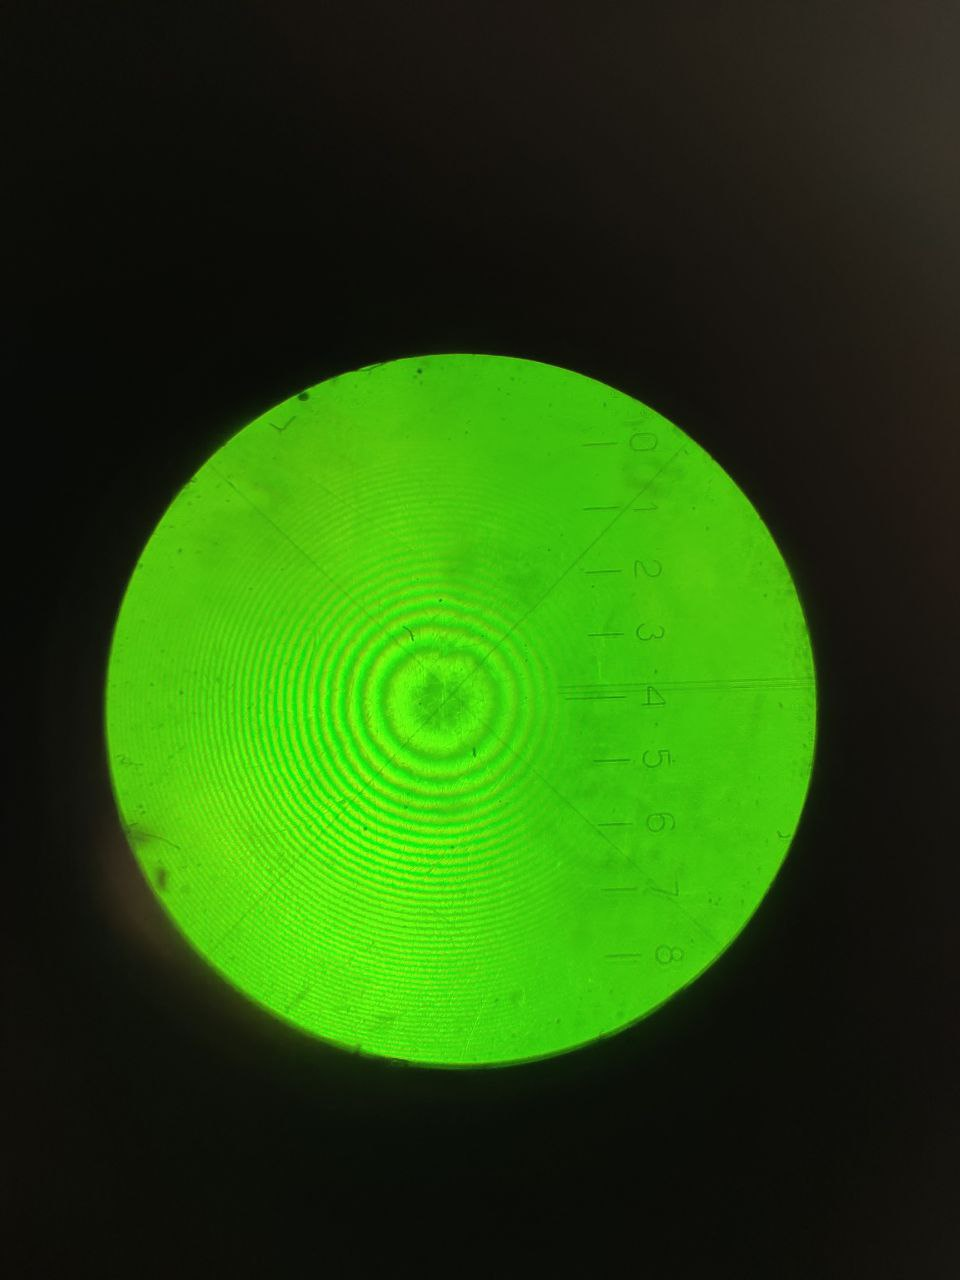
\includegraphics[width=12cm]{images/picture.jpg}
    \caption{Наблюдение биений}
\end{figure}

Получив картину биений, просчитаем количество тёмных полос $\Delta m$ от центра одной чёткой системы полос до центра соседней чёткой системы.

Мы наблюдали следующее количество полос между центрами четких систем $\Delta m = 12$. Вычислим отсюда разность длин волн желтого и зеленого света ртутной лампы $\Delta \lambda = \lambda_{\text{ж}} - \lambda_{\text{3}}$:

$$
(\Delta m + 1)\lambda_{\text{3}} = \Delta m\lambda_{\text{ж}} \Rightarrow \Delta \lambda = \frac{\lambda_{\text{3}}}{\Delta m} \approx {45}{\text{ нм}}
$$

Теоретическое значение для разности длин волн желтой и зеленой линии спектра около $\Delta \lambda = \lambda_{\text{ж}} - \lambda_{\text{3}} = 40$ нм.


\section*{Вывод}
1) Измерили радиус светлых и темных колец Ньютона.\\\indent
2) Определили радиус кривизны линзы. \\\indent
3) По картине биений рассчитали разность длин волн желтой и зеленой линий спектра ртутной лампы $\labmda = 45$ нм. Табличное значение - 40 нм.

